\documentclass{article}
\usepackage{tikz}
\usepackage{amssymb}
\pagestyle{empty}
\begin{document}
% GEOMIRA export: TikZ. One unit is 50bp (66.666667 px on screen).
% Needs \usepackage{tikz} and \usepackage{amssymb}.
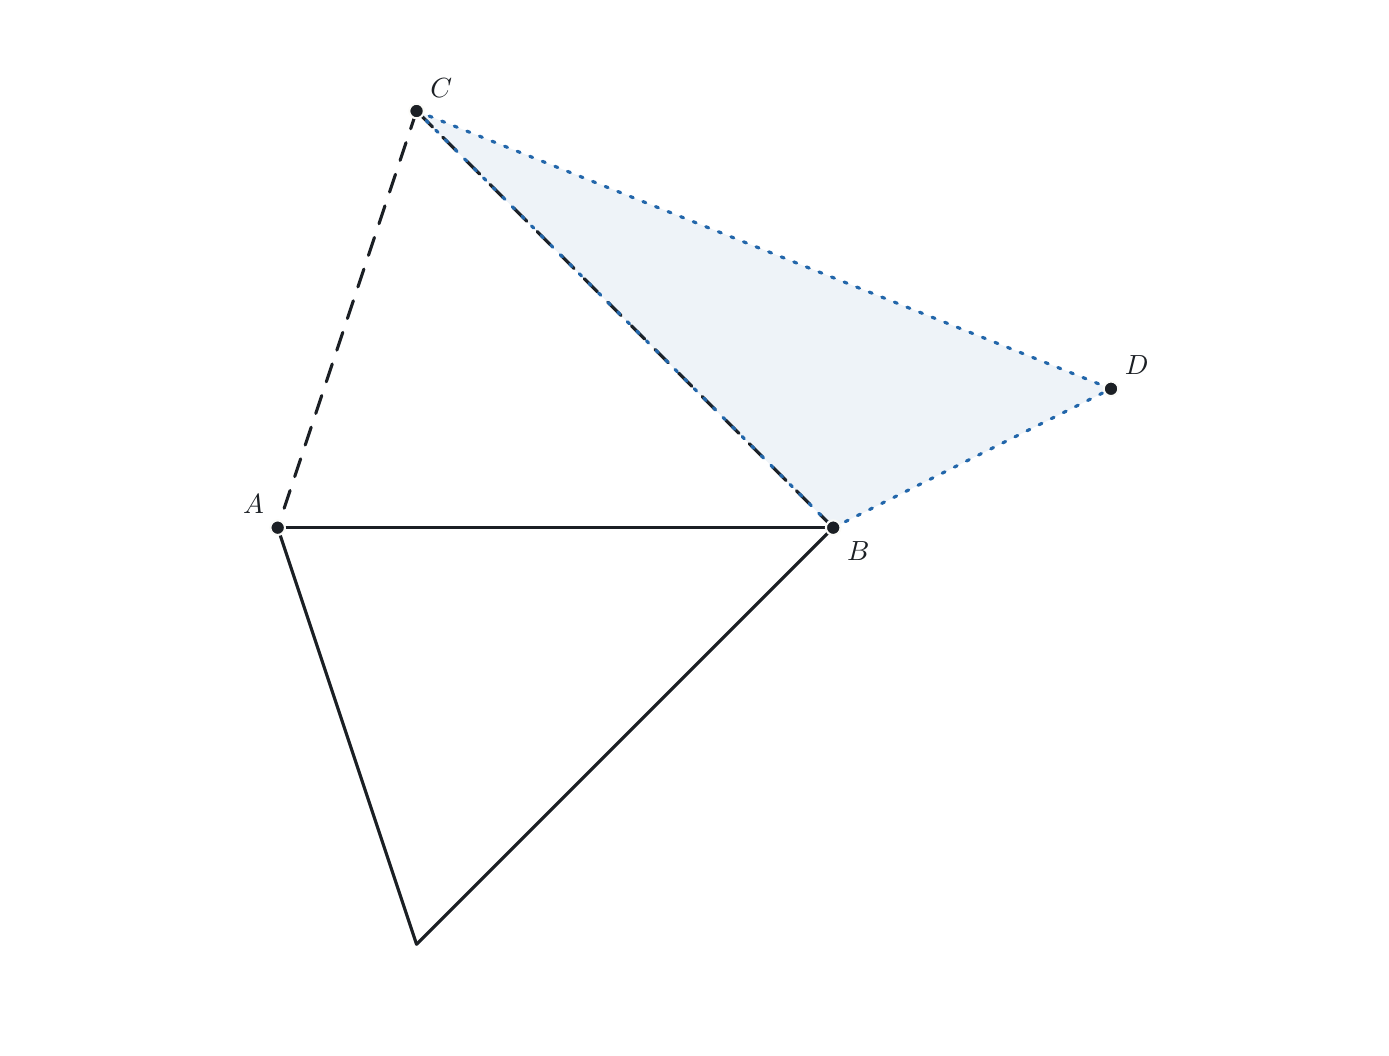
\begin{tikzpicture}[x=50bp, y=50bp, line cap=round, line join=round]
\definecolor{gmc0}{HTML}{1B1F24}
\definecolor{gmc1}{HTML}{2266AA}
\definecolor{gmc2}{HTML}{FBFBF8}
\clip (-1.8,-3.6) rectangle (7.8,3.6);
% t
\draw[gmc0, line width=1.125bp, dash pattern=on 6.75bp off 5.25bp] (0,0) -- (4,0);
\draw[gmc0, line width=1.125bp, dash pattern=on 6.75bp off 5.25bp] (4,0) -- (1,3);
\draw[gmc0, line width=1.125bp, dash pattern=on 6.75bp off 5.25bp] (1,3) -- (0,0);
% u
\fill[gmc1, fill opacity=0.08] (4,0) -- (6,1) -- (1,3) -- cycle;
\draw[gmc1, line width=1.125bp, dash pattern=on 1.125bp off 3.75bp] (4,0) -- (6,1);
\draw[gmc1, line width=1.125bp, dash pattern=on 1.125bp off 3.75bp] (6,1) -- (1,3);
\draw[gmc1, line width=1.125bp, dash pattern=on 1.125bp off 3.75bp] (1,3) -- (4,0);
% r
\draw[gmc0, line width=1.125bp] (0,0) -- (4,0);
\draw[gmc0, line width=1.125bp] (4,0) -- (1,-3);
\draw[gmc0, line width=1.125bp] (1,-3) -- (0,0);
% A
\filldraw[fill=gmc0, draw=gmc2, line width=0.75bp] (0,0) circle[radius=2.625bp];
% B
\filldraw[fill=gmc0, draw=gmc2, line width=0.75bp] (4,0) circle[radius=2.625bp];
% C
\filldraw[fill=gmc0, draw=gmc2, line width=0.75bp] (1,3) circle[radius=2.625bp];
% D
\filldraw[fill=gmc0, draw=gmc2, line width=0.75bp] (6,1) circle[radius=2.625bp];
\node[anchor=south east, inner sep=0pt, text=gmc0] at (-0.0955,0.0955) {$A$}; % label of A
\node[anchor=north west, inner sep=0pt, text=gmc0] at (4.0955,-0.0955) {$B$}; % label of B
\node[anchor=south west, inner sep=0pt, text=gmc0] at (1.0955,3.0955) {$C$}; % label of C
\node[anchor=south west, inner sep=0pt, text=gmc0] at (6.0955,1.0955) {$D$}; % label of D
\end{tikzpicture}

\end{document}
